\chapter{Serving, Quantization, and Cost}
\label{ch:serving-quantization-cost}
\raggedbottom

In 2023, the vLLM paper reported a result that looked less glamorous than a new benchmark record but mattered just as much for real users: by changing how the KV cache was managed, the serving system improved throughput by roughly $2$--$4\times$ over strong baselines at similar latency~\cite{kwon2023pagedattention}. The model weights were not better. The prompts were not smarter. The post-training recipe did not change. The system simply wasted less memory while serving many variable-length requests.

That is the central shock of serving. Once a model is trained, deployment quality is not only about model quality. A good model can feel slow, expensive, or unreliable if the runtime cannot schedule requests, store KV caches, batch decode steps, and fit the chosen precision on available hardware. Conversely, a careful serving stack can make the same model usable in settings where a naive implementation would time out or run out of memory.

Chapter~\ref{ch:inference-time-scaling} treated inference-time compute as an algorithmic resource: sample more, vote, verify, search. This chapter asks the systems question underneath that algorithmic story:

\begin{quote}
How do we make those runtime procedures affordable enough to use?
\end{quote}

\paragraph{Chapter thesis.} \emph{Serving turns a model into a resource-allocation problem: weights, KV cache, requests, batches, precision, latency, and dollars must all fit at once.} Model quality matters, but the deployed system's value depends on throughput, time-to-first-token, time-per-output-token, memory headroom, and cost per useful task.

\paragraph{Running example.} Suppose your Project~4 assistant uses a 7B model. In a notebook, one user sends one prompt and waits. In production, many users send prompts of different lengths, some ask for short answers, some ask for long reasoning traces, and some use best-of-$N$ from Chapter~\ref{ch:inference-time-scaling}. The model is the same. The serving problem is not. A single-user demo asks, ``can the model answer?'' A serving system asks, ``how many answers per second, at what latency, with what memory, and at what cost?''

\subsection*{Learning Objectives}

After completing this chapter, you should be able to:

\begin{enumerate}
  \item Distinguish prompt prefill cost, per-token decode cost, time-to-first-token, and time-per-output-token.
  \item Estimate memory consumed by model weights and KV cache under different context lengths and precisions.
  \item Explain why continuous batching improves throughput for variable-length generation.
  \item Describe why PagedAttention and prefix reuse matter for serving, not just implementation elegance.
  \item Compare weight-only quantization, weight-activation quantization, and KV-cache quantization.
  \item Reason about speculative decoding as latency reduction rather than quality improvement.
  \item Report cost per useful task rather than only tokens per second.
\end{enumerate}

\subsection*{Notation}

\begin{center}
\begin{tabularx}{\textwidth}{@{}lX@{}}
\toprule
Symbol & Meaning \\
\midrule
$B$ & Number of active sequences in a batch \\
$L_{\text{in}}$, $L_{\text{out}}$ & Input prompt tokens and generated output tokens \\
$T$ & Total cached sequence length for one request \\
$L$ & Number of Transformer layers \\
$n_{\text{kv}}$ & Number of key/value heads after MHA, GQA, or MQA choices \\
$d_k$ & Dimension of one key/value head \\
$b_w$, $b_{\text{kv}}$ & Bytes per weight parameter and bytes per KV-cache element \\
$\lambda$ & Request arrival rate, usually requests per second \\
\bottomrule
\end{tabularx}
\end{center}

\subsection*{Timeline of Key Contributions}

\begin{center}
\begin{tabularx}{\textwidth}{@{}lX@{}}
\toprule
\textbf{Year} & \textbf{Milestone} \\
\midrule
2022 & FlashAttention shows that attention kernels can be reorganized around memory IO, changing practical speed without changing model math~\cite{dao2022flashattention}. \\
2022 & Orca introduces iteration-level scheduling and selective batching for generative Transformer serving~\cite{yu2022orca}. \\
2022 & GPTQ studies accurate post-training quantization for GPT-style models~\cite{frantar2022gptq}. \\
2022 & SmoothQuant makes weight-and-activation INT8 quantization practical for large language models~\cite{xiao2023smoothquant}. \\
2023 & Speculative decoding shows how a small draft model can reduce serial decode latency while preserving the target distribution~\cite{leviathan2023speculative}. \\
2023 & vLLM introduces PagedAttention for memory-efficient KV-cache management~\cite{kwon2023pagedattention}. \\
2024 & SGLang studies efficient execution for structured LLM programs with runtime support for caching, batching, and control flow~\cite{zheng2024sglang}. \\
\bottomrule
\end{tabularx}
\end{center}

\paragraph{What this chapter covers.} We begin with the serving timeline of one request: prompt prefill, per-token execution, and user-visible latency. This is not a reintroduction to autoregressive generation or sampling; earlier chapters already covered that. Here the point is systems accounting. We then turn to the memory budget, where weights and KV cache compete for the same GPU. Next we study batching and scheduling, because real services run many uneven requests at once. The second half covers quantization, speculative decoding as a latency optimization, and the final cost model: not ``how fast is the model?'' but ``how much does one successful task cost?''


%----------------------------------------------------------------------
\section{The Serving View of Generation}
\label{sec:ch19-serving-view}

Chapter~\ref{ch:decoder-only} introduced the autoregressive GPT loop and the KV cache: the model repeatedly predicts the next token while reusing cached keys and values from earlier positions. Chapter~\ref{ch:inference-time-scaling} used \emph{decoding} in the algorithmic sense: choosing outputs through greedy decoding, sampling, best-of-$N$, voting, verification, or search. This chapter uses the word in a narrower systems sense. \emph{Decode} means the per-token execution phase after the prompt has already been processed and cached.

Serving combines those earlier ideas with a queue of users, a fixed hardware budget, and a target latency. The first step is not to reteach how GPT generates text, but to separate two runtime phases that feel identical to a user and stress the GPU differently: prompt prefill and per-token decode.

\subsection{Prompt Prefill and Per-Token Decode}

\textbf{Prefill} is the serving name for the initial forward pass over the input prompt. If a user sends a 4{,}000-token prompt, the runtime processes those prompt tokens, fills the KV cache for them, and produces logits for the first generated token. This stage is often compute-heavy: many matrix multiplications can run efficiently as large parallel kernels.

\textbf{Decode}, in this chapter's serving terminology, is the repeated one-token execution phase after prefill. Each step appends one token's key and value vectors to the cache and attends over the growing history. This phase is sequential across generated tokens. It is often memory-bandwidth-heavy because every new token must read a large amount of cached state.

Two user-visible metrics follow naturally:

\begin{itemize}[nosep]
  \item \textbf{Time to first token (TTFT)}: how long the user waits before the response begins. Long prompts and cold caches mostly affect this.
  \item \textbf{Time per output token (TPOT)}: how quickly later tokens stream after generation begins. Decode scheduling, batch size, and KV-cache movement mostly affect this.
\end{itemize}

In the Project~4 assistant, a retrieval-heavy prompt may have high TTFT because it sends many context tokens into prefill. A reasoning-heavy answer may have high TPOT cost because it generates hundreds or thousands of tokens. Treating both as ``latency'' hides the engineering choice. The relevant question is no longer ``which token should the model sample next?'' from Chapter~\ref{ch:inference-time-scaling}; it is ``where does this request spend wall-clock time and GPU memory?''

\subsection{Throughput Is Not Latency}

Throughput measures how much work the system completes per unit time: tokens per second, requests per second, or successful tasks per hour. Latency measures how long one request waits. They are related but not interchangeable. A large batch can improve GPU utilization and throughput while making an individual request wait longer. A single-request path can minimize latency while wasting hardware.

This tension is the serving version of the Ch18 cost--reliability frontier. Ch18 asked whether extra samples improve reliability enough to justify their cost. Ch19 asks whether the serving stack can process those samples without destroying latency.

\subsection{The Restaurant Analogy}

A useful analogy is a restaurant kitchen. Prefill is like reading and preparing the whole order ticket. Per-token decode is like plating the meal one item at a time while the customer is watching. Batching is cooking several compatible dishes together. KV-cache memory is counter space: even if the chefs are fast, the kitchen stalls when too many half-finished plates occupy the counter.

The analogy is imperfect, but it captures the serving mindset. A system is not only the recipe. It is the kitchen layout, the queue, the counter space, and the policy for deciding which ticket gets attention next.

\begin{figure}[t]
\centering
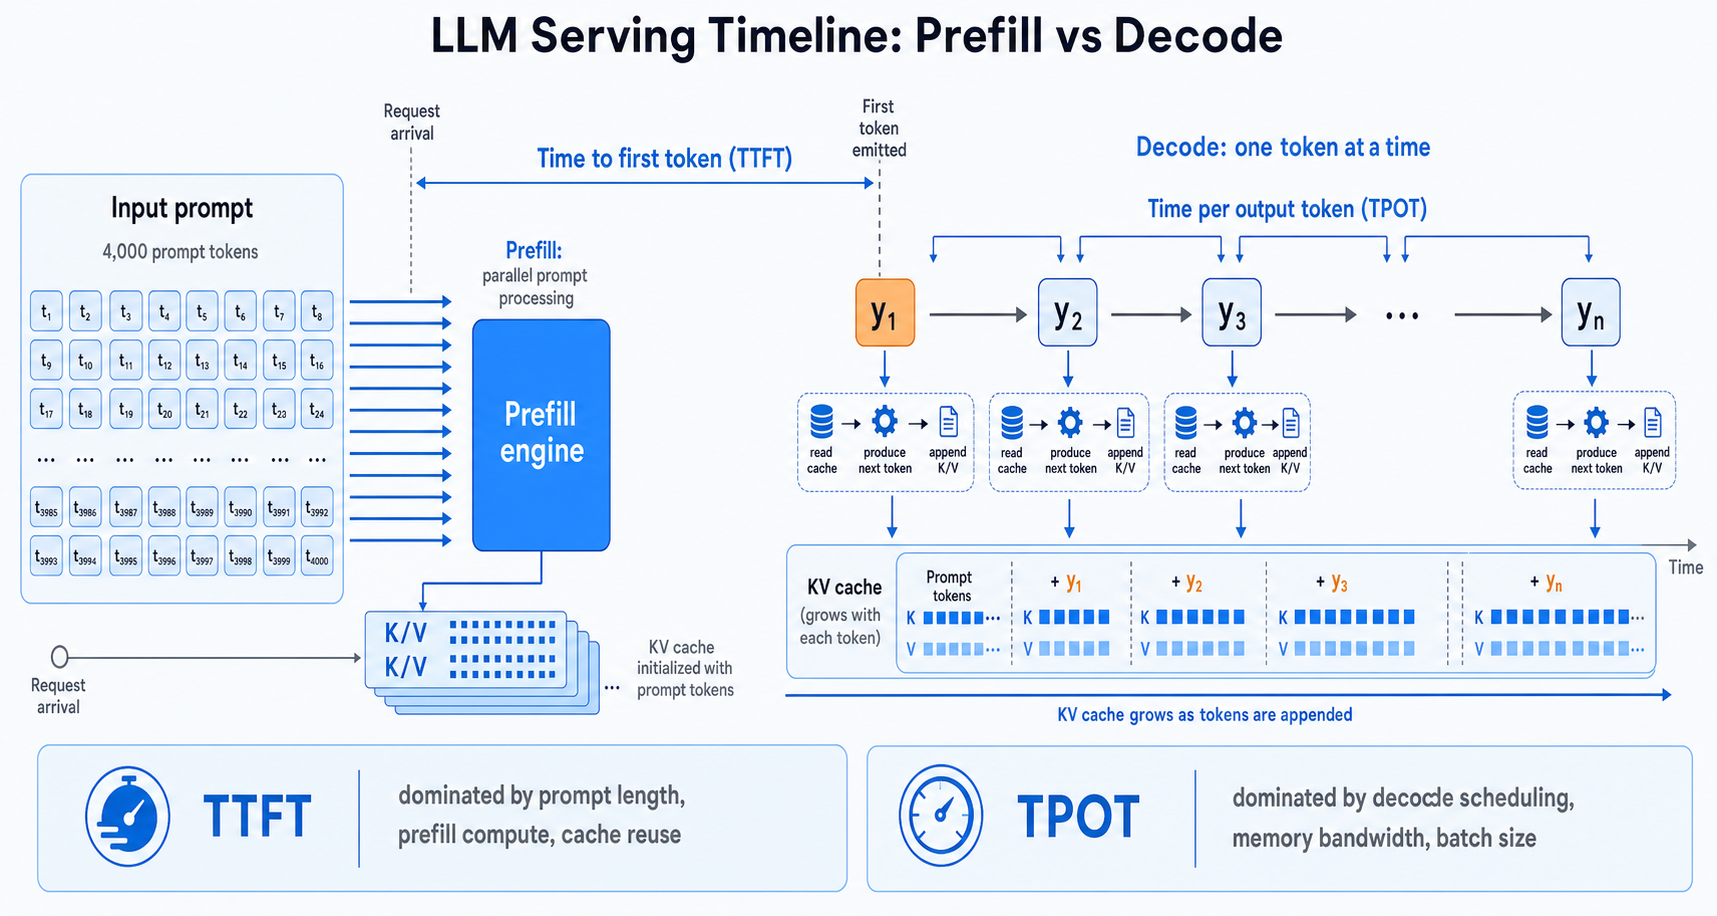
\includegraphics[width=0.95\textwidth]{figures/ch19/fig_prefill_decode_timeline.png}
\caption{\textbf{Prefill and per-token decode in one request.} Prefill processes the full prompt and fills the KV cache before the first token appears. The serving decode phase then streams tokens sequentially, appending new K/V entries at each step. TTFT and TPOT diagnose different bottlenecks.}
\label{fig:ch19-prefill-decode-timeline}
\end{figure}

\begin{quickrecap}
\textbf{Quick Recap.}
\begin{itemize}[nosep,leftmargin=1.5em]
  \item Prefill handles the input prompt in parallel; serving decode executes one generated token step at a time.
  \item TTFT and TPOT should be reported separately.
  \item Throughput and latency trade off through batching, scheduling, and hardware utilization.
\end{itemize}
\textit{Next: the first hard constraint is memory, especially the KV cache.}
\end{quickrecap}


%----------------------------------------------------------------------
\section{Memory Budgets: Weights, Activations, and KV Cache}
\label{sec:ch19-memory}

The serving memory budget has a different shape from the training memory budget in Chapter~\ref{ch:what-changes}. Training must store weights, gradients, optimizer states, and activations for backpropagation. Inference drops gradients and optimizer states, but it adds a dynamic object that grows with each active request: the KV cache.

\subsection{The Weight Footprint}

For a dense model with $P$ parameters, the raw weight memory is approximately

\begin{equation}
  M_{\text{weights}} \approx P \cdot b_w.
  \label{eq:ch19-weight-memory}
\end{equation}

A 7B model in bf16 uses about $7 \times 10^9 \times 2 \approx 14$\,GB for weights before runtime overhead. In 8-bit weight format, the raw footprint is about 7\,GB. In 4-bit weight format, it is about 3.5\,GB plus scales, zero points, packing overhead, and kernel-specific metadata.

This is why a 7B model can be easy to load but still hard to serve well. Loading weights is only the beginning. The remaining memory determines batch size, context length, number of concurrent users, and whether best-of-$N$ from Chapter~\ref{ch:inference-time-scaling} is practical.

\subsection{The KV-Cache Footprint}

Chapter~\ref{ch:decoder-only} gave the basic KV-cache formula. In serving notation, one request with cached length $T$ consumes roughly

\begin{equation}
  M_{\text{KV, one request}}
  \approx 2 \cdot L \cdot n_{\text{kv}} \cdot T \cdot d_k \cdot b_{\text{kv}}.
  \label{eq:ch19-kv-memory-one}
\end{equation}

For a batch of variable-length requests, sum this over active requests:

\begin{equation}
  M_{\text{KV, batch}}
  \approx \sum_{i=1}^{B}
  2 \cdot L \cdot n_{\text{kv}} \cdot T_i \cdot d_k \cdot b_{\text{kv}}.
  \label{eq:ch19-kv-memory-batch}
\end{equation}

The dependence on $T_i$ is the important part. Long prompts and long generations consume cache. Many short chats may fit; a few long-context reasoning sessions may evict everything else. GQA and MQA help because they reduce $n_{\text{kv}}$, shrinking the cache without shrinking the number of query heads.

\noindent\fbox{\parbox{\dimexpr\textwidth-2\fboxsep-2\fboxrule\relax}{\textbf{Pause and verify.} Consider a 32-layer model with $n_{\text{kv}}=8$, $d_k=128$, and bf16 KV cache ($b_{\text{kv}}=2$ bytes). Estimate the KV cache for one 8K-token request:
\[
2 \cdot 32 \cdot 8 \cdot 8192 \cdot 128 \cdot 2 \text{ bytes}.
\]
Now multiply by 32 concurrent requests. Which is larger: the 14\,GB bf16 weights of a 7B model, or the batch KV cache?}}

\subsection{Fragmentation and the PagedAttention Idea}

The simple formula assumes perfect packing. Real serving is messier. Requests arrive at different times, have different prompt lengths, and finish after different numbers of output tokens. If the runtime reserves one contiguous cache region per request, memory can fragment: enough total memory exists, but not in the right contiguous shape.

PagedAttention addresses this by borrowing an operating-system idea: store KV cache in fixed-size blocks and map logical sequence positions to physical blocks~\cite{kwon2023pagedattention}. This makes cache allocation more flexible and allows sharing blocks across requests that share prefixes. vLLM is the serving engine built around this idea.

The conceptual lesson is broader than vLLM. In serving, memory management is an algorithmic part of model quality. A model that theoretically fits may fail to serve useful workloads if the KV cache wastes memory.

\begin{figure}[t]
\centering
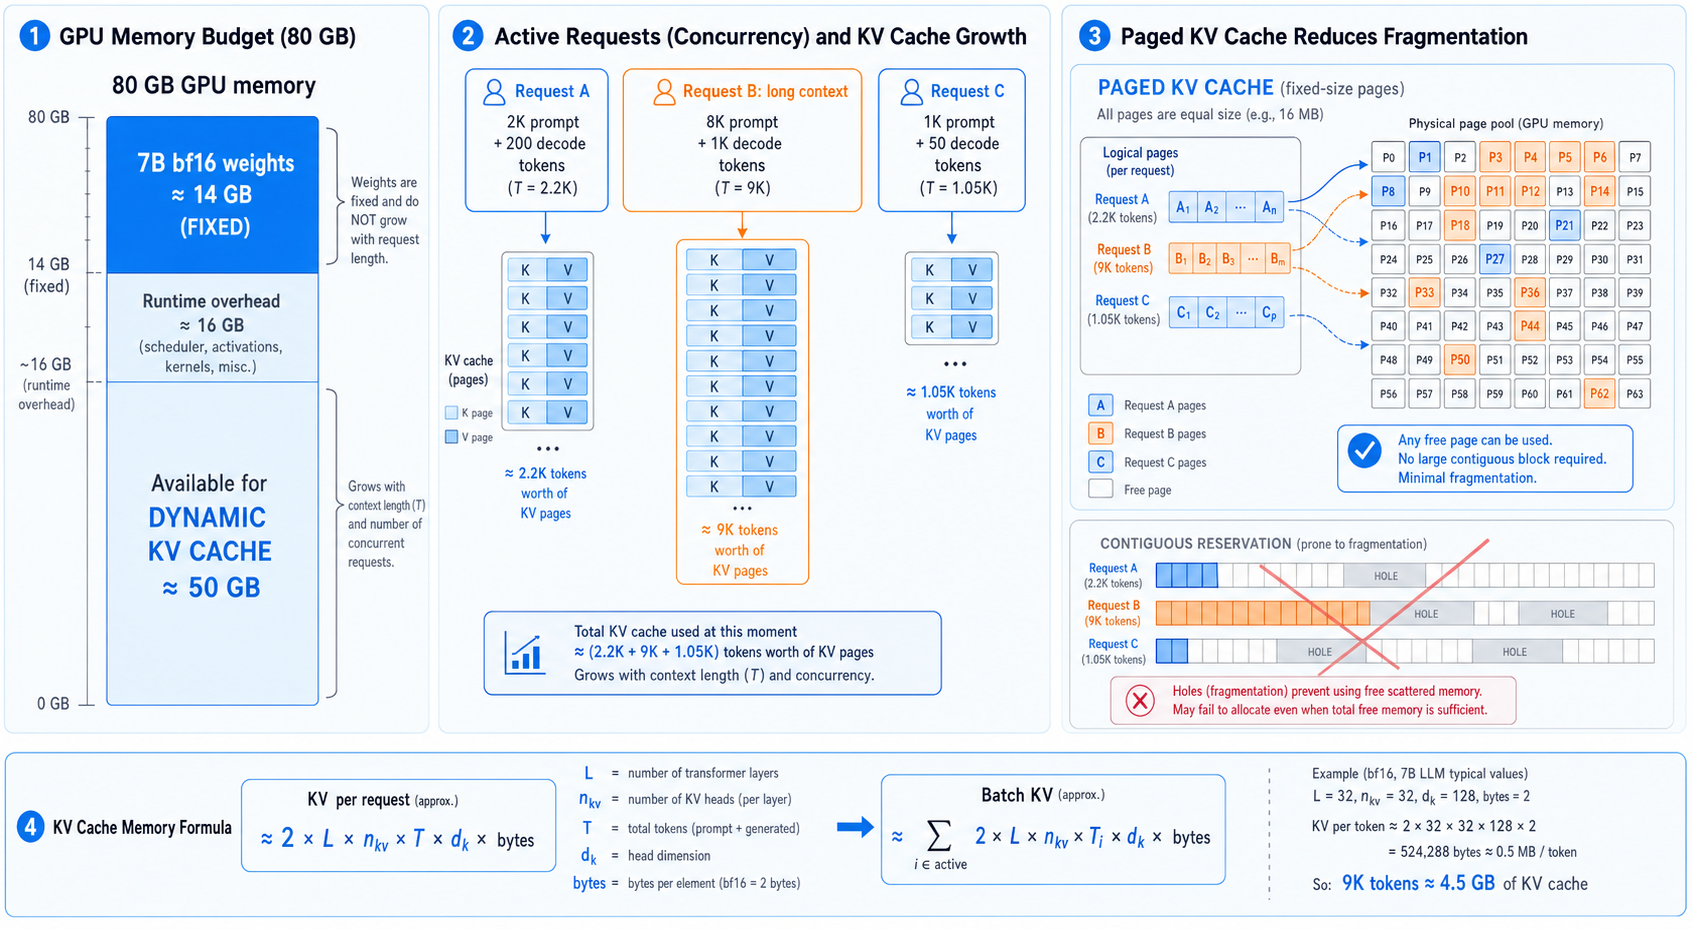
\includegraphics[width=0.95\textwidth]{figures/ch19/fig_memory_budget_kv_cache.png}
\caption{\textbf{Serving memory budget.} Weights occupy a fixed block; KV cache grows with active requests, context length, and generated tokens. Paged KV-cache management reduces fragmentation by storing sequences in reusable blocks rather than requiring one contiguous region per request.}
\label{fig:ch19-memory-budget-kv-cache}
\end{figure}

\begin{tcolorbox}[colback=gray!8, colframe=gray!40, title=\textbf{Echo from Ch3: KV Cache Changes Role}]
In Chapter~\ref{ch:decoder-only}, the KV cache was an algorithmic trick: avoid recomputing old keys and values during autoregressive generation. In this chapter, the same cache becomes a product constraint. It determines how many users fit, how long their contexts can be, and how expensive Ch18-style multiple-sample inference becomes.
\end{tcolorbox}

\begin{quickrecap}
\textbf{Quick Recap.}
\begin{itemize}[nosep,leftmargin=1.5em]
  \item Inference removes optimizer and gradient memory but adds dynamic KV-cache memory.
  \item Weight memory is mostly fixed; KV memory scales with active requests and context length.
  \item Paged KV-cache management matters because variable-length requests fragment memory.
\end{itemize}
\textit{Next: once memory fits, scheduling determines whether the GPU stays busy.}
\end{quickrecap}


%----------------------------------------------------------------------
\section{Batching, Scheduling, and Serving Engines}
\label{sec:ch19-batching}

GPUs are efficient when work arrives in large enough batches. Autoregressive generation is awkward because different requests have different prompt lengths, output lengths, and stop times. A naive server might wait for a batch of requests, run each request until completion, then start the next batch. That wastes capacity whenever some sequences finish early and others keep decoding.

\subsection{Static Batching}

In static batching, the server groups requests and processes the group together. This is simple and effective when requests are similar. It fails when output lengths vary. If one request finishes after 20 tokens and another runs for 800 tokens, either the short request wastes padding or the system needs special logic to remove it.

Static batching also creates queueing delay. If the system waits too long to form a large batch, TTFT worsens. If it uses tiny batches to reduce waiting, GPU utilization worsens. The serving problem is therefore not only model execution; it is online scheduling under uncertain future lengths.

\subsection{Continuous Batching}

Continuous batching, also called iteration-level scheduling in Orca, updates the active batch at each decode step~\cite{yu2022orca}. Finished sequences leave. New requests can enter. The GPU processes one decode iteration for the current active set, then the scheduler updates the set again.

This is a better match for autoregressive serving because decode is naturally stepwise. Instead of treating a request as one long indivisible job, the runtime treats generation as a sequence of small scheduling opportunities.

For the Project~4 assistant, continuous batching matters when some users ask short factual questions and others ask long tool-planning analyses. Without continuous batching, long generations can trap capacity. With it, short requests can join the active set between decode steps.

\subsection{Prefix Reuse and Structured Programs}

Many workloads share prefixes: a system prompt, a tool schema, a retrieved document header, or a few-shot template. Prefix caching stores the KV cache for a common prefix so later requests can reuse it rather than recompute it. This improves TTFT when prompts share large fixed components.

SGLang extends this systems view to structured language model programs: multi-call workflows, branches, constraints, and shared context fragments~\cite{zheng2024sglang}. The exact tool will change, but the idea will not. Once LLM applications become programs rather than single calls, the runtime must understand reuse, control flow, and batching opportunities across calls.

\begin{figure}[t]
\centering
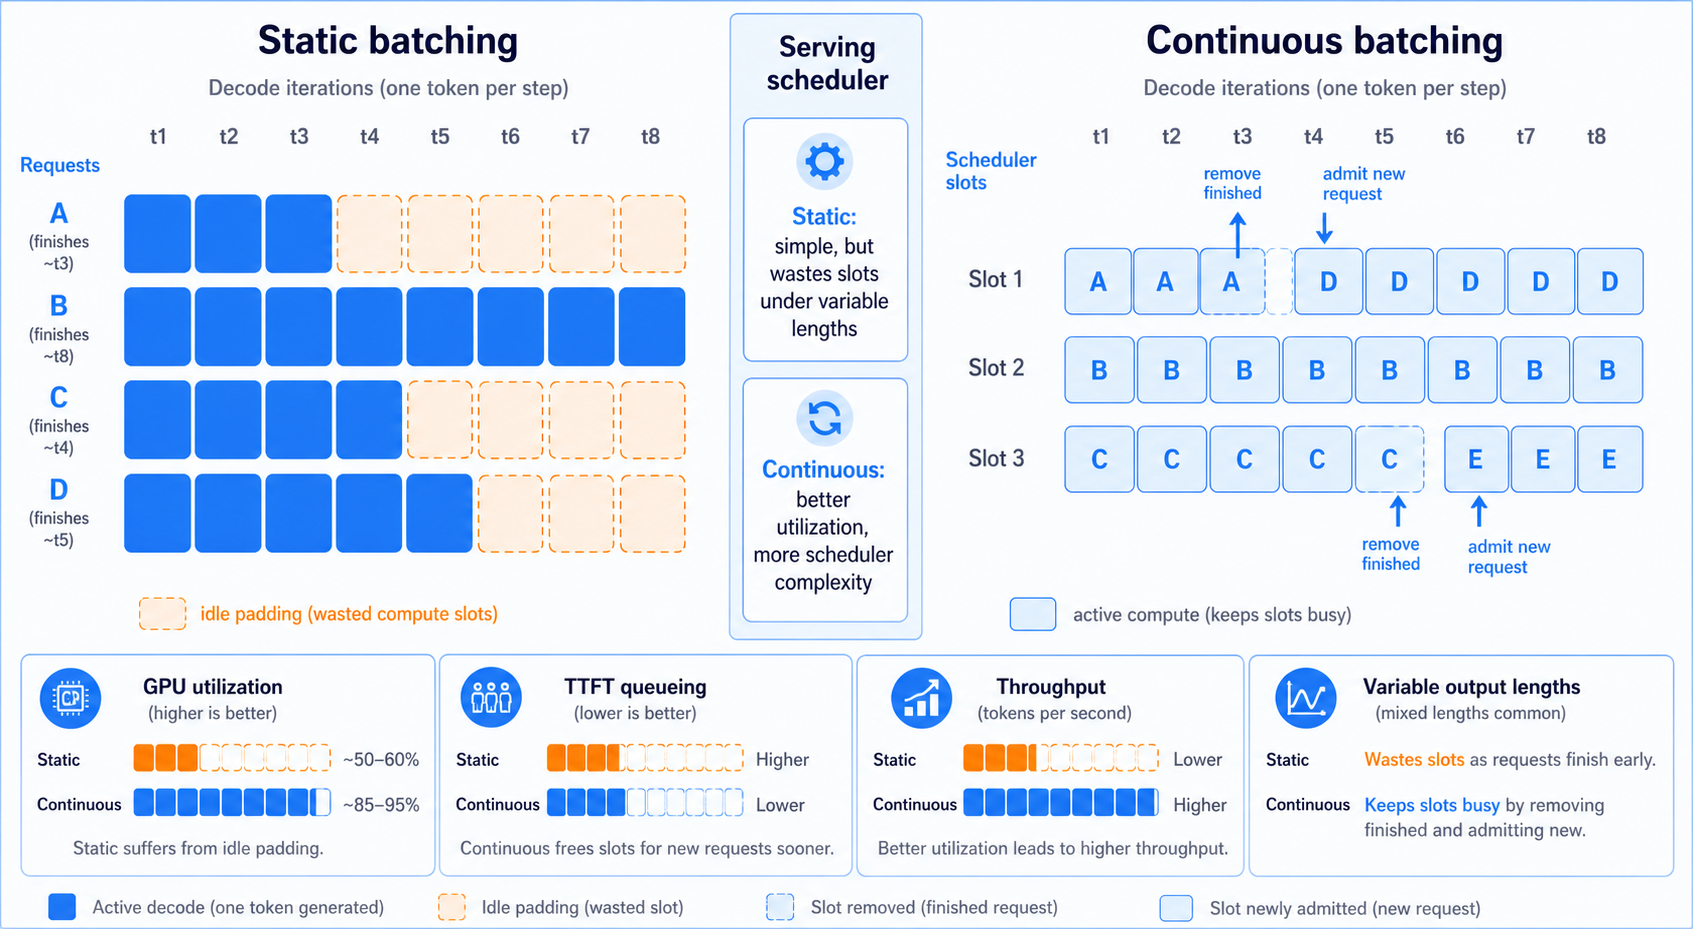
\includegraphics[width=0.95\textwidth]{figures/ch19/fig_continuous_batching.png}
\caption{\textbf{Static versus continuous batching.} Static batching holds a group until completion, wasting slots as sequences finish at different lengths. Continuous batching updates the active set at each decode step, admitting new requests and removing completed ones.}
\label{fig:ch19-continuous-batching}
\end{figure}

\begin{tcolorbox}[colback=blue!5, colframe=blue!40, title=\textbf{Is Serving Just Engineering?}]
It is engineering, but not ``just'' engineering. Serving choices change which research ideas are usable. A verifier from Chapter~\ref{ch:inference-time-scaling} may improve accuracy but be impossible under a 500\,ms latency budget. A long-context method from Chapter~\ref{ch:long-context-retrieval-memory} may work in a paper and fail in a multi-user system because KV cache dominates memory. Systems constraints decide which model behaviors reach users.
\end{tcolorbox}

\begin{quickrecap}
\textbf{Quick Recap.}
\begin{itemize}[nosep,leftmargin=1.5em]
  \item Static batching is simple but brittle under variable output lengths.
  \item Continuous batching treats each decode step as a scheduling opportunity.
  \item Prefix reuse and structured runtime support matter when applications make repeated or programmatic model calls.
\end{itemize}
\textit{Next: quantization changes the memory and bandwidth terms directly.}
\end{quickrecap}


%----------------------------------------------------------------------
\section{Quantization for Serving}
\label{sec:ch19-quantization}

Quantization appeared in Chapter~\ref{ch:peft} through QLoRA: compress the frozen base so adapter tuning fits on smaller hardware. Serving uses quantization for a related but distinct goal. The question is not only ``can the model fit?'' It is also ``does lower precision improve throughput, reduce memory bandwidth, or allow more concurrent requests without unacceptable quality loss?''

\subsection{What Gets Quantized?}

There are three common targets:

\begin{enumerate}[nosep]
  \item \textbf{Weights}: compress model parameters. Weight-only 8-bit or 4-bit quantization reduces model memory and weight bandwidth.
  \item \textbf{Activations}: quantize intermediate values used during matmuls. Weight-and-activation schemes such as W8A8 can map well to hardware kernels, but activation outliers make them harder.
  \item \textbf{KV cache}: store cached keys and values in lower precision. This directly increases context and batch capacity, but can affect attention quality over long contexts.
\end{enumerate}

Different methods choose different compromises. GPTQ uses approximate second-order information for post-training weight quantization~\cite{frantar2022gptq}. AWQ protects salient weights identified through activation behavior and is commonly used for weight-only low-bit serving~\cite{lin2024awq}. SmoothQuant shifts difficulty from activation quantization into weights, making W8A8 inference more practical~\cite{xiao2023smoothquant}. QLoRA's NF4 is excellent for finetuning a frozen base, but serving stacks often care just as much about kernel support and throughput as compression ratio~\cite{dettmers2023qlora}.

\subsection{Quality Loss Is Task-Dependent}

Quantization error is not a single number. A 4-bit model may look fine on short chat, degrade on math, and degrade more on long-context retrieval. Tool use can be brittle because one wrong JSON character or tool argument may cause a full task failure. Safety and calibration may shift in ways that are not visible in a small perplexity check.

This is why Project~4 should measure output quality under the same task harness used for the unquantized model. If quantization doubles throughput but increases tool-call failures by 10\%, the serving improvement may or may not be worth it depending on the product target.

\subsection{The Kernel Reality}

Quantization only helps if the hardware and kernels can exploit it. A compressed format that must be dequantized inefficiently may save memory while failing to improve latency. A format with mature fused kernels may improve both memory and throughput. This is why serving reports should name not only the bit width but also the backend, kernel path, GPU type, batch size, context length, and workload.

\begin{figure}[t]
\centering
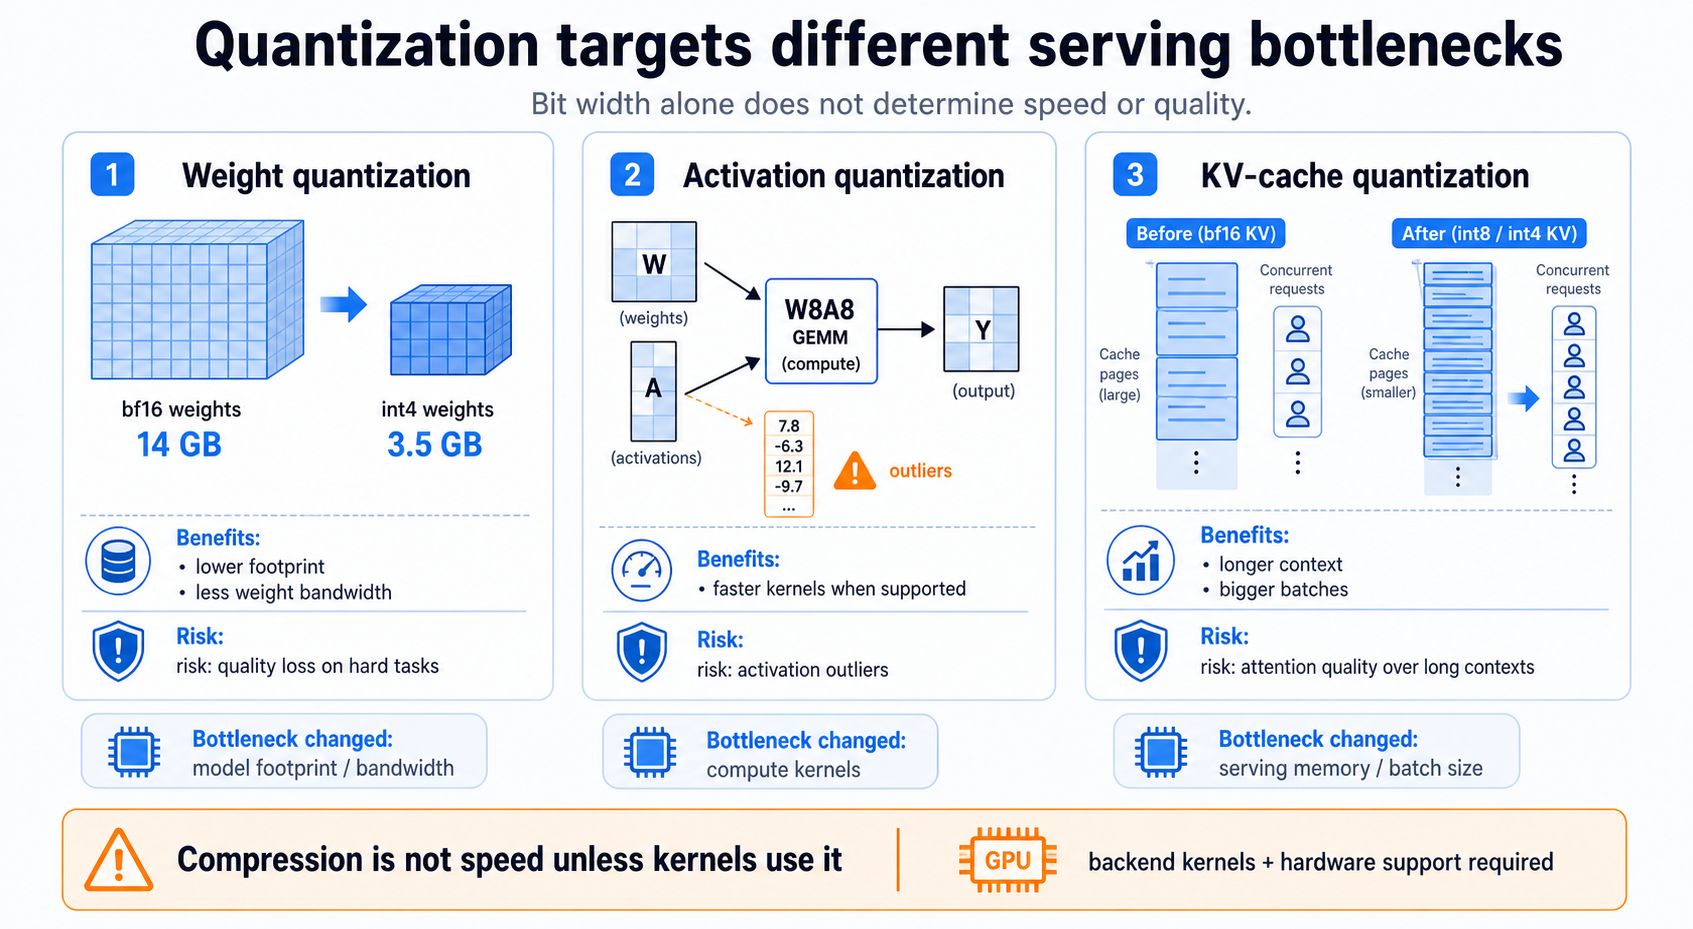
\includegraphics[width=0.95\textwidth]{figures/ch19/fig_quantization_tradeoffs.png}
\caption{\textbf{Quantization targets for serving.} Weight quantization reduces model footprint; activation quantization can accelerate matmuls when kernels support it; KV-cache quantization expands batch and context capacity. Each target has a different quality and systems risk.}
\label{fig:ch19-quantization-tradeoffs}
\end{figure}

\noindent\fbox{\parbox{\dimexpr\textwidth-2\fboxsep-2\fboxrule\relax}{\textbf{Pause and verify.} A 13B model in bf16 uses about 26\,GB for weights. A 4-bit weight-only version uses about 6.5\,GB before metadata. Suppose the saved 19.5\,GB is used for bf16 KV cache. Using the KV formula from Section~\ref{sec:ch19-memory}, estimate how many additional 8K-token requests fit for a model with $L=40$, $n_{\text{kv}}=8$, and $d_k=128$. What hidden assumptions make this estimate optimistic?}}

\begin{quickrecap}
\textbf{Quick Recap.}
\begin{itemize}[nosep,leftmargin=1.5em]
  \item Weight quantization, activation quantization, and KV-cache quantization solve different serving problems.
  \item Compression ratio is not the same as speed; kernel support determines practical gains.
  \item Quantization quality must be measured on the deployed task, not only perplexity or generic chat.
\end{itemize}
\textit{Next: some latency gains come from changing the serving decode path rather than the precision.}
\end{quickrecap}


%----------------------------------------------------------------------
\section{Speculative Decoding and Latency Reduction}
\label{sec:ch19-speculative}

The serving decode phase is serial: token 101 cannot be generated by the target model until token 100 is known. Speculative decoding attacks this latency by using a cheaper draft model to propose several tokens, then asking the expensive target model to verify them in parallel~\cite{leviathan2023speculative}. The name is unfortunate for this book's sequence: here again, \emph{decoding} means a runtime execution path, not the Ch18 question of whether to use greedy sampling, top-$p$, best-of-$N$, or a verifier.

\subsection{Draft, Verify, Accept}

The basic loop is:

\begin{enumerate}[nosep]
  \item A small draft model proposes several future tokens.
  \item The large target model evaluates those proposed tokens in a single parallel pass.
  \item Tokens that match the target distribution are accepted; the first rejected token triggers correction.
  \item The process repeats from the new prefix.
\end{enumerate}

If the draft model is close to the target model, many tokens are accepted and the system reduces wall-clock decode time. If the draft model is poor, verification rejects many tokens and the overhead may not pay off.

\subsection{What It Does Not Do}

Speculative decoding is easy to misread as a quality method. It is not best-of-$N$, not verifier reranking, and not self-consistency. In its distribution-preserving form, it aims to produce the same distribution as ordinary target-model decoding, only faster. Its purpose is latency reduction.

This distinction matters for Ch18. Ch18 methods often improve reliability by spending extra compute. Speculative decoding tries to reduce the latency of producing the same kind of sample. It is a serving method, not an inference-time reasoning method, even though both live at runtime.

\subsection{When It Helps}

Speculative decoding helps when the target model is expensive, the draft model is cheap, and the draft model's proposals are often accepted. It is less useful when the target model is already small, when batch scheduling dominates latency, when prompts are prefill-heavy rather than decode-heavy, or when the draft model disagrees often.

For the Project~4 assistant, speculative decoding might speed up long natural-language answers. It is less likely to fix a tool-use failure or improve a math answer. It changes the speed of generation, not the correctness criterion.

\begin{figure}[t]
\centering
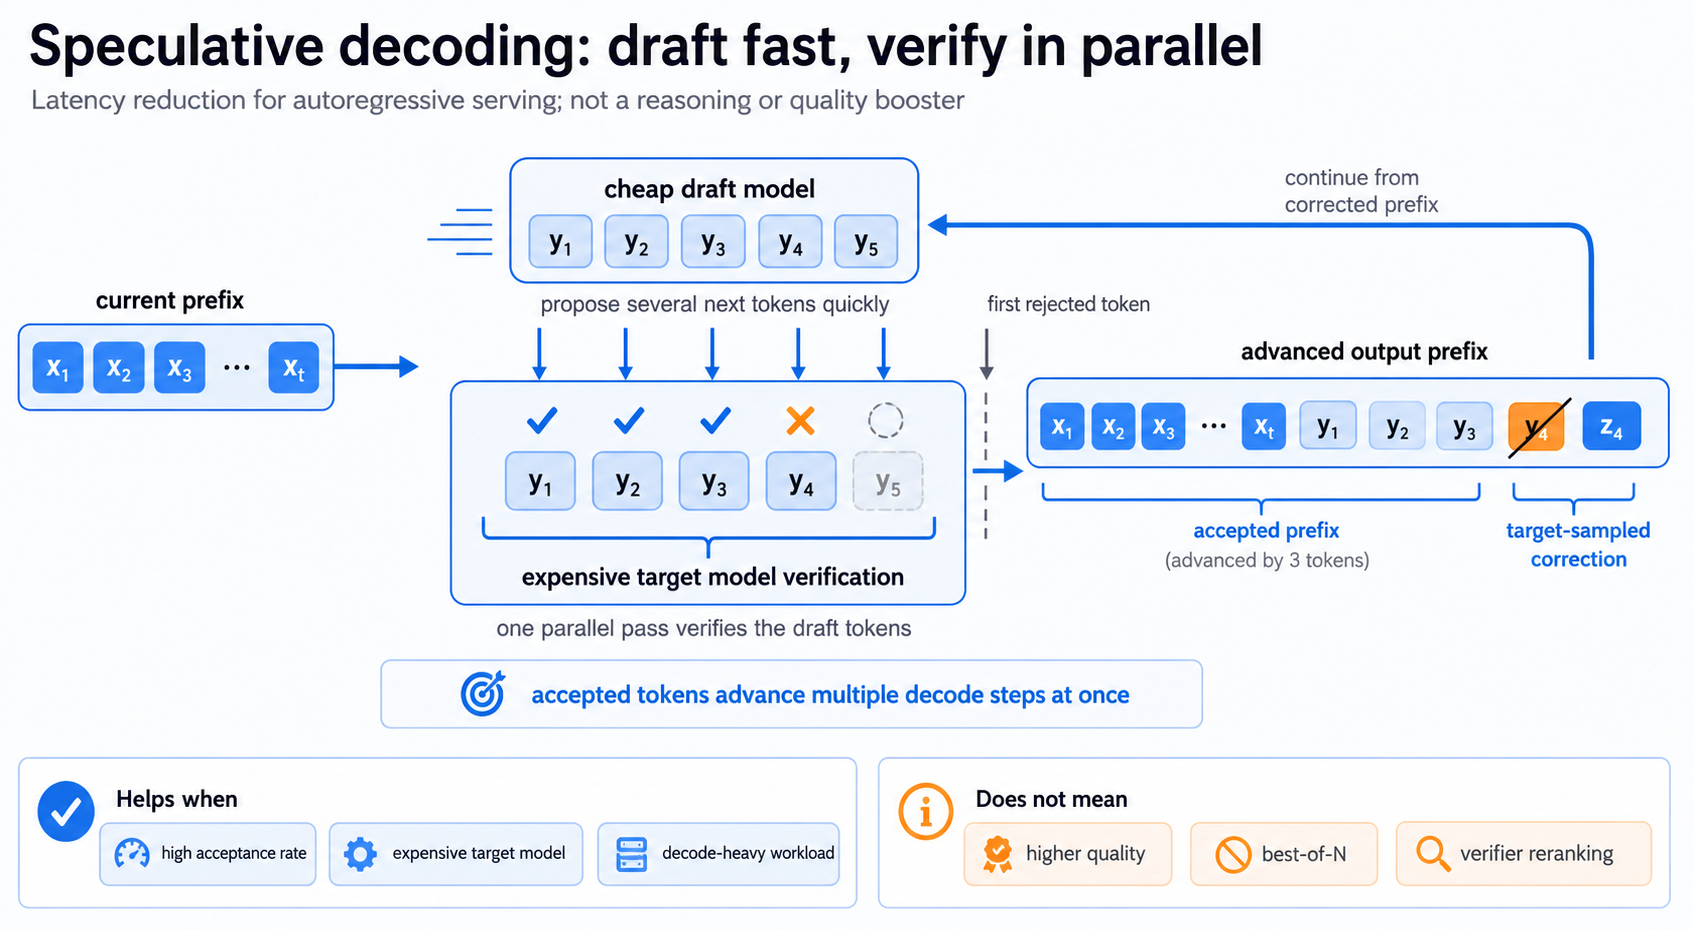
\includegraphics[width=0.95\textwidth]{figures/ch19/fig_speculative_decoding.png}
\caption{\textbf{Speculative decoding.} A small draft model proposes multiple future tokens. The target model verifies them in parallel and accepts a prefix of the draft when it matches the target distribution. The gain is lower decode latency, not new reasoning capability.}
\label{fig:ch19-speculative-decoding}
\end{figure}

\begin{quickrecap}
\textbf{Quick Recap.}
\begin{itemize}[nosep,leftmargin=1.5em]
  \item Speculative decoding uses a cheap draft model and an expensive target model.
  \item Its goal is faster decoding, not better answers.
  \item It helps only when accepted draft tokens are common enough to pay for the draft and verification overhead.
\end{itemize}
\textit{Next: all serving choices must finally be reported as cost per useful task.}
\end{quickrecap}


%----------------------------------------------------------------------
\section{Cost per Useful Task}
\label{sec:ch19-cost}

Tokens per second is a useful systems metric. It is not the final product metric. A system can generate many low-quality tokens cheaply, or produce one correct tool-mediated answer expensively. Part~IV therefore needs a metric that connects serving to task success.

\subsection{A Simple Cost Model}

For a rough serving estimate, separate input tokens, output tokens, number of samples, and verification or tool calls:

\begin{equation}
  C_{\text{request}}
  \approx
  C_{\text{prefill}}(L_{\text{in}})
  + N \cdot C_{\text{decode}}(L_{\text{out}})
  + C_{\text{extra}},
  \label{eq:ch19-request-cost}
\end{equation}

where $N$ is the number of candidates from Ch18 and $C_{\text{extra}}$ includes verifier calls, tool calls, retrieval, reranking, or additional model passes. This equation is intentionally simplified. Real billing may depend on GPU rental, utilization, tokens, reserved capacity, networking, and engineering overhead. But the decomposition prevents a common mistake: reporting the cost of one model call when the actual system makes many calls.

If task success rate is $s$, then a crude cost per successful task is

\begin{equation}
  C_{\text{success}} \approx \frac{C_{\text{request}}}{s}.
  \label{eq:ch19-cost-success}
\end{equation}

This makes reliability and serving cost inseparable. A cheap system with 20\% success may cost more per success than an expensive system with 80\% success. A quantized model that is faster but less reliable may or may not improve the final metric.

\subsection{Operating Points}

Every deployed system chooses an operating point:

\begin{itemize}[nosep]
  \item \textbf{Low-latency chat}: small $N$, conservative max tokens, strong batching discipline.
  \item \textbf{Batch coding assistant}: larger $N$, test execution, reranking, looser latency.
  \item \textbf{RAG assistant}: higher prefill cost, prefix caching, retrieval and reranking overhead.
  \item \textbf{Agent loop}: multiple model calls, tool latency, retries, trace logging, and failure attribution.
\end{itemize}

The same model can be reasonable in one operating point and wrong in another. This is why serving belongs before long context, tools, and agent evaluation in Part~IV. The later systems chapters all inherit this cost structure.

\subsection{What to Report}

A serious serving report should include:

\begin{itemize}[nosep]
  \item model name, parameter count, precision, quantization method, and backend;
  \item GPU type, number of GPUs, tensor/pipeline parallelism if used;
  \item prompt length distribution, output length distribution, and max context;
  \item TTFT, TPOT, tokens/sec, requests/sec, batch size, and concurrency;
  \item task success, failure categories, and quality changes under quantization;
  \item cost per request and cost per successful task.
\end{itemize}

For Project~4, this report is more important than a single demo transcript. It tells you whether the system can survive realistic workload pressure.

\begin{figure}[t]
\centering
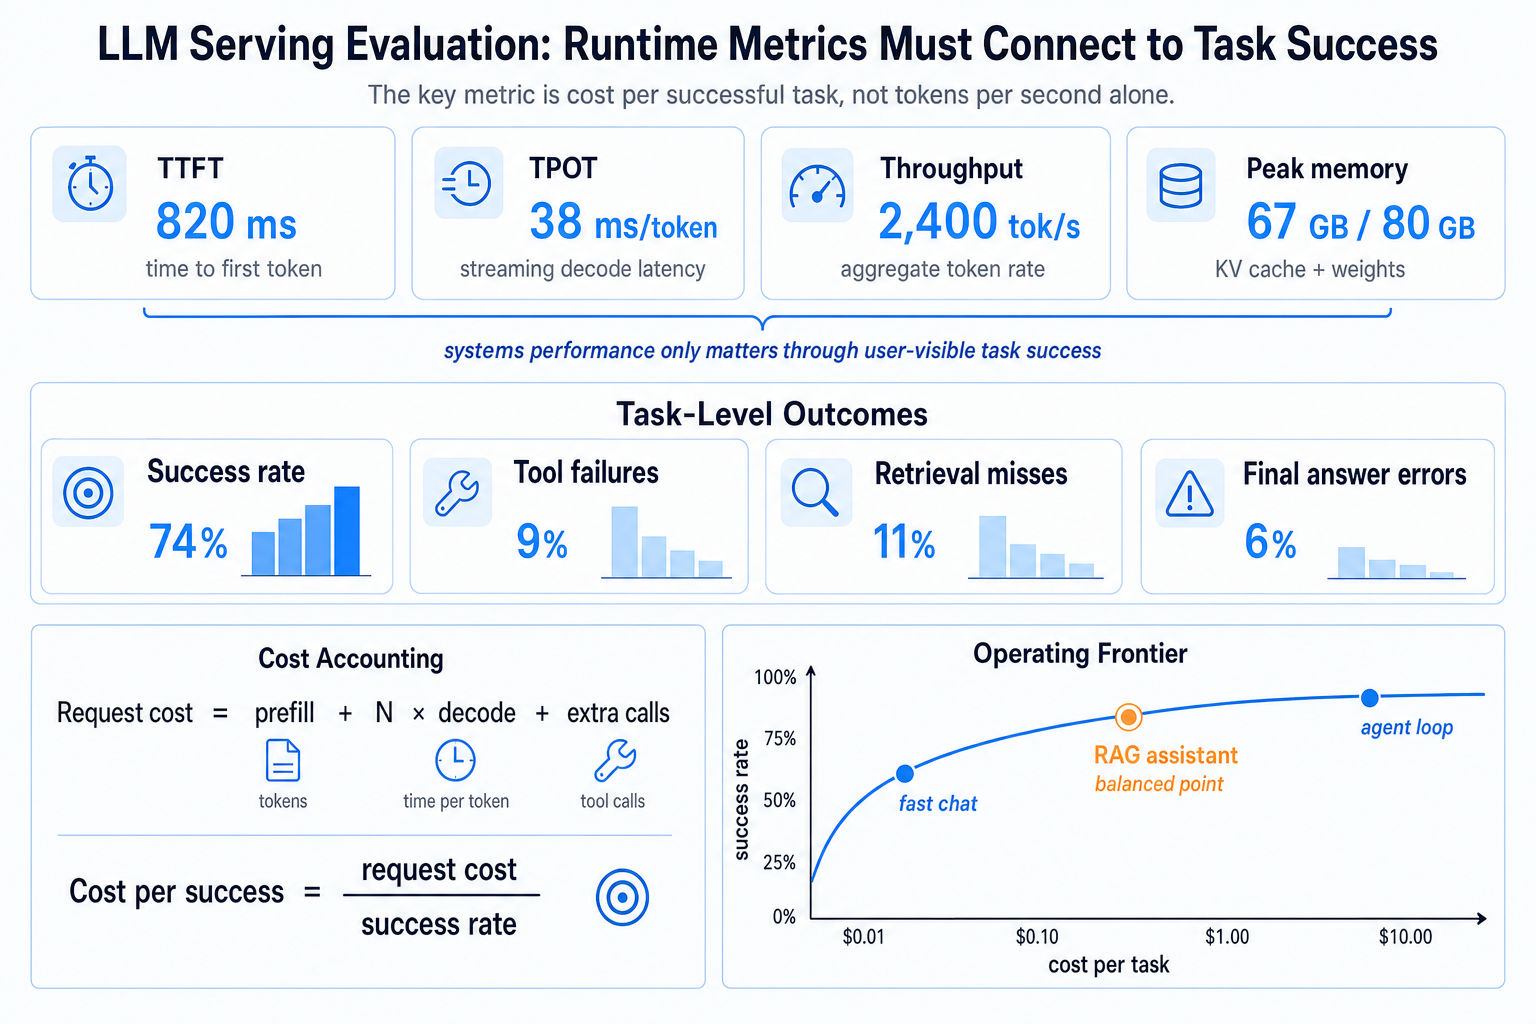
\includegraphics[width=0.95\textwidth]{figures/ch19/fig_cost_reliability_dashboard.png}
\caption{\textbf{Cost per useful task dashboard.} A serving report should connect systems metrics (TTFT, TPOT, throughput, memory) to task metrics (success rate and failure type). The relevant frontier is cost per successful task, not maximum tokens per second alone.}
\label{fig:ch19-cost-reliability-dashboard}
\end{figure}

\begin{tcolorbox}[colback=orange!5, colframe=orange!60, title=\textbf{For Project~4: Benchmark the System, Not the Call}]
When comparing a plain assistant, RAG assistant, tool workflow, and agent loop, keep a serving sheet beside the task sheet:
\begin{itemize}[nosep,leftmargin=1.4em]
  \item TTFT and TPOT for each system variant.
  \item Total model calls, input tokens, output tokens, and verifier or tool calls.
  \item Peak memory or maximum concurrency if you run locally.
  \item Cost per attempted task and cost per successful task.
\end{itemize}
The goal is not to make the cheapest system. It is to know what reliability costs.
\end{tcolorbox}

\begin{quickrecap}
\textbf{Quick Recap.}
\begin{itemize}[nosep,leftmargin=1.5em]
  \item Request cost includes prefill, per-token decode, repeated candidates, and extra model or tool calls.
  \item Cost per success can favor a more expensive but more reliable system.
  \item Serving reports should connect hardware metrics to task outcomes.
\end{itemize}
\textit{Next: Ch20 changes the prompt itself by adding long context, retrieval, and memory.}
\end{quickrecap}


%----------------------------------------------------------------------
% End matter
%----------------------------------------------------------------------

\begin{takeaways}
\begin{enumerate}
  \item Serving separates prompt prefill from per-token decode; TTFT and TPOT diagnose different bottlenecks.
  \item Inference memory is dominated by weights plus a dynamic KV cache that scales with context length and concurrency.
  \item Paged KV-cache management reduces memory waste for variable-length requests.
  \item Continuous batching improves throughput by scheduling at the decode-iteration level.
  \item Quantization can reduce memory and bandwidth, but quality and speed gains depend on task, precision target, kernels, and hardware.
  \item Speculative decoding reduces decode latency when draft tokens are accepted often enough.
  \item The final systems metric is cost per useful task, not tokens per second alone.
\end{enumerate}
\end{takeaways}


\section*{Summary}

\paragraph{What this chapter established.} Ch19 turned inference from an algorithmic idea into a deployment resource budget. The same fixed model can be fast or slow, cheap or expensive, scalable or memory-bound depending on prefill/decode behavior, KV-cache management, batching, precision, scheduling, and request mix.

\paragraph{The kitchen lesson.} Serving is the kitchen around the model. The recipe matters, but the number of cooks, counter space, order queue, batch cooking policy, and plating speed determine whether customers get useful meals on time. In LLM terms: weights matter, but KV cache, batching, quantization, and latency budgets decide which model behaviors can actually be delivered.

\paragraph{One sentence.} \emph{A served model is a memory- and scheduling-constrained system for converting tokens, cache, and GPU time into successful tasks.}

\paragraph{What comes next.} Chapter~\ref{ch:long-context-retrieval-memory} asks what happens when the input context itself becomes part of the system: long prompts, retrieval, compression, attribution, and external memory.

\section*{Key Equations}

\begin{center}
\small
\begin{tabularx}{\textwidth}{@{}p{3.6cm}p{5.4cm}X@{}}
\toprule
\textbf{Equation} & \textbf{Form} & \textbf{Why it matters} \\
\midrule
Weight memory & $M_{\text{weights}} \approx P b_w$ & Fixed model footprint before runtime overhead. \\
Single-request KV cache & $M_{\text{KV}} \approx 2Ln_{\text{kv}}Td_kb_{\text{kv}}$ & Context length and GQA/MQA choices directly determine cache size. \\
Batch KV cache & $M_{\text{KV,batch}} \approx \sum_i 2Ln_{\text{kv}}T_id_kb_{\text{kv}}$ & Variable-length requests make memory a scheduling problem. \\
Request cost & $C_{\text{request}} \approx C_{\text{prefill}} + N C_{\text{decode}} + C_{\text{extra}}$ & Ch18 sampling and verification multiply serving cost. \\
Cost per success & $C_{\text{success}} \approx C_{\text{request}}/s$ & Reliability and serving cost must be evaluated together. \\
\bottomrule
\end{tabularx}
\normalsize
\end{center}

\section*{Key Checks}

\begin{center}
\small
\begin{tabularx}{\textwidth}{@{}p{3.8cm}p{5.2cm}X@{}}
\toprule
\textbf{Diagnostic} & \textbf{Question} & \textbf{Action} \\
\midrule
Latency split & Are TTFT and TPOT reported separately? & Diagnose prefill-heavy and decode-heavy bottlenecks differently. \\
Memory budget & How much memory is weights versus KV cache at target concurrency? & Estimate both before choosing context length or batch size. \\
Batching policy & Does the server use static or continuous batching? & Test under variable output lengths, not only uniform synthetic prompts. \\
Quantization audit & What precision target changed, and did task quality change? & Report backend, kernels, hardware, and task-level deltas. \\
Speculation fit & Are draft tokens accepted often enough to pay for overhead? & Measure acceptance rate and end-to-end latency, not just draft speed. \\
Cost per success & Does a cheaper request remain cheaper after failures and retries? & Divide total system cost by successful task count. \\
\bottomrule
\end{tabularx}
\normalsize
\end{center}


\section*{Key Readings}

\begin{enumerate}[nosep]
  \item \textbf{Dao et al., 2022.} ``FlashAttention''~\cite{dao2022flashattention}. The canonical example of changing practical attention speed by changing IO-aware kernel structure rather than model math.
  \item \textbf{Yu et al., 2022.} ``Orca''~\cite{yu2022orca}. Introduced iteration-level scheduling and selective batching for generative Transformer serving.
  \item \textbf{Frantar et al., 2022.} ``GPTQ''~\cite{frantar2022gptq}. A key post-training quantization method for GPT-style models.
  \item \textbf{Xiao et al., 2023.} ``SmoothQuant''~\cite{xiao2023smoothquant}. Shows how to make W8A8 quantization practical by smoothing activation outliers into weights.
  \item \textbf{Leviathan et al., 2023.} ``Fast Inference from Transformers via Speculative Decoding''~\cite{leviathan2023speculative}. The core distribution-preserving draft-and-verify latency method.
  \item \textbf{Kwon et al., 2023.} ``Efficient Memory Management for LLM Serving with PagedAttention''~\cite{kwon2023pagedattention}. The vLLM/PagedAttention paper that made KV-cache memory management central.
  \item \textbf{Zheng et al., 2024.} ``SGLang''~\cite{zheng2024sglang}. A runtime and programming model for efficient structured language model programs.
\end{enumerate}

\flushbottom
